% Options for packages loaded elsewhere
\PassOptionsToPackage{unicode}{hyperref}
\PassOptionsToPackage{hyphens}{url}
\PassOptionsToPackage{dvipsnames,svgnames,x11names}{xcolor}
%
\documentclass[
  12pt,
  a4paper,
]{article}
\usepackage{amsmath,amssymb}
\usepackage{lmodern}
\usepackage{setspace}
\usepackage{iftex}
\ifPDFTeX
  \usepackage[T1]{fontenc}
  \usepackage[utf8]{inputenc}
  \usepackage{textcomp} % provide euro and other symbols
\else % if luatex or xetex
  \usepackage{unicode-math}
  \defaultfontfeatures{Scale=MatchLowercase}
  \defaultfontfeatures[\rmfamily]{Ligatures=TeX,Scale=1}
\fi
% Use upquote if available, for straight quotes in verbatim environments
\IfFileExists{upquote.sty}{\usepackage{upquote}}{}
\IfFileExists{microtype.sty}{% use microtype if available
  \usepackage[]{microtype}
  \UseMicrotypeSet[protrusion]{basicmath} % disable protrusion for tt fonts
}{}
\makeatletter
\@ifundefined{KOMAClassName}{% if non-KOMA class
  \IfFileExists{parskip.sty}{%
    \usepackage{parskip}
  }{% else
    \setlength{\parindent}{0pt}
    \setlength{\parskip}{6pt plus 2pt minus 1pt}}
}{% if KOMA class
  \KOMAoptions{parskip=half}}
\makeatother
\usepackage{xcolor}
\usepackage[left=2.54cm,right=2.54cm,top=2.54cm,bottom=2.54cm]{geometry}
\usepackage{color}
\usepackage{fancyvrb}
\newcommand{\VerbBar}{|}
\newcommand{\VERB}{\Verb[commandchars=\\\{\}]}
\DefineVerbatimEnvironment{Highlighting}{Verbatim}{commandchars=\\\{\}}
% Add ',fontsize=\small' for more characters per line
\usepackage{framed}
\definecolor{shadecolor}{RGB}{248,248,248}
\newenvironment{Shaded}{\begin{snugshade}}{\end{snugshade}}
\newcommand{\AlertTok}[1]{\textcolor[rgb]{0.94,0.16,0.16}{#1}}
\newcommand{\AnnotationTok}[1]{\textcolor[rgb]{0.56,0.35,0.01}{\textbf{\textit{#1}}}}
\newcommand{\AttributeTok}[1]{\textcolor[rgb]{0.77,0.63,0.00}{#1}}
\newcommand{\BaseNTok}[1]{\textcolor[rgb]{0.00,0.00,0.81}{#1}}
\newcommand{\BuiltInTok}[1]{#1}
\newcommand{\CharTok}[1]{\textcolor[rgb]{0.31,0.60,0.02}{#1}}
\newcommand{\CommentTok}[1]{\textcolor[rgb]{0.56,0.35,0.01}{\textit{#1}}}
\newcommand{\CommentVarTok}[1]{\textcolor[rgb]{0.56,0.35,0.01}{\textbf{\textit{#1}}}}
\newcommand{\ConstantTok}[1]{\textcolor[rgb]{0.00,0.00,0.00}{#1}}
\newcommand{\ControlFlowTok}[1]{\textcolor[rgb]{0.13,0.29,0.53}{\textbf{#1}}}
\newcommand{\DataTypeTok}[1]{\textcolor[rgb]{0.13,0.29,0.53}{#1}}
\newcommand{\DecValTok}[1]{\textcolor[rgb]{0.00,0.00,0.81}{#1}}
\newcommand{\DocumentationTok}[1]{\textcolor[rgb]{0.56,0.35,0.01}{\textbf{\textit{#1}}}}
\newcommand{\ErrorTok}[1]{\textcolor[rgb]{0.64,0.00,0.00}{\textbf{#1}}}
\newcommand{\ExtensionTok}[1]{#1}
\newcommand{\FloatTok}[1]{\textcolor[rgb]{0.00,0.00,0.81}{#1}}
\newcommand{\FunctionTok}[1]{\textcolor[rgb]{0.00,0.00,0.00}{#1}}
\newcommand{\ImportTok}[1]{#1}
\newcommand{\InformationTok}[1]{\textcolor[rgb]{0.56,0.35,0.01}{\textbf{\textit{#1}}}}
\newcommand{\KeywordTok}[1]{\textcolor[rgb]{0.13,0.29,0.53}{\textbf{#1}}}
\newcommand{\NormalTok}[1]{#1}
\newcommand{\OperatorTok}[1]{\textcolor[rgb]{0.81,0.36,0.00}{\textbf{#1}}}
\newcommand{\OtherTok}[1]{\textcolor[rgb]{0.56,0.35,0.01}{#1}}
\newcommand{\PreprocessorTok}[1]{\textcolor[rgb]{0.56,0.35,0.01}{\textit{#1}}}
\newcommand{\RegionMarkerTok}[1]{#1}
\newcommand{\SpecialCharTok}[1]{\textcolor[rgb]{0.00,0.00,0.00}{#1}}
\newcommand{\SpecialStringTok}[1]{\textcolor[rgb]{0.31,0.60,0.02}{#1}}
\newcommand{\StringTok}[1]{\textcolor[rgb]{0.31,0.60,0.02}{#1}}
\newcommand{\VariableTok}[1]{\textcolor[rgb]{0.00,0.00,0.00}{#1}}
\newcommand{\VerbatimStringTok}[1]{\textcolor[rgb]{0.31,0.60,0.02}{#1}}
\newcommand{\WarningTok}[1]{\textcolor[rgb]{0.56,0.35,0.01}{\textbf{\textit{#1}}}}
\usepackage{longtable,booktabs,array}
\usepackage{calc} % for calculating minipage widths
% Correct order of tables after \paragraph or \subparagraph
\usepackage{etoolbox}
\makeatletter
\patchcmd\longtable{\par}{\if@noskipsec\mbox{}\fi\par}{}{}
\makeatother
% Allow footnotes in longtable head/foot
\IfFileExists{footnotehyper.sty}{\usepackage{footnotehyper}}{\usepackage{footnote}}
\makesavenoteenv{longtable}
\setlength{\emergencystretch}{3em} % prevent overfull lines
\providecommand{\tightlist}{%
  \setlength{\itemsep}{0pt}\setlength{\parskip}{0pt}}
\setcounter{secnumdepth}{-\maxdimen} % remove section numbering
\newlength{\cslhangindent}
\setlength{\cslhangindent}{1.5em}
\newlength{\csllabelwidth}
\setlength{\csllabelwidth}{3em}
\newlength{\cslentryspacingunit} % times entry-spacing
\setlength{\cslentryspacingunit}{\parskip}
\newenvironment{CSLReferences}[2] % #1 hanging-ident, #2 entry spacing
 {% don't indent paragraphs
  \setlength{\parindent}{0pt}
  % turn on hanging indent if param 1 is 1
  \ifodd #1
  \let\oldpar\par
  \def\par{\hangindent=\cslhangindent\oldpar}
  \fi
  % set entry spacing
  \setlength{\parskip}{#2\cslentryspacingunit}
 }%
 {}
\usepackage{calc}
\newcommand{\CSLBlock}[1]{#1\hfill\break}
\newcommand{\CSLLeftMargin}[1]{\parbox[t]{\csllabelwidth}{#1}}
\newcommand{\CSLRightInline}[1]{\parbox[t]{\linewidth - \csllabelwidth}{#1}\break}
\newcommand{\CSLIndent}[1]{\hspace{\cslhangindent}#1}
\ifLuaTeX
\usepackage[bidi=basic]{babel}
\else
\usepackage[bidi=default]{babel}
\fi
\babelprovide[main,import]{english}
% get rid of language-specific shorthands (see #6817):
\let\LanguageShortHands\languageshorthands
\def\languageshorthands#1{}
\usepackage{titling}
\pretitle{\begin{center}\LARGE
\includegraphics[width=7cm]{../img/logo_isuc.png}\\[\bigskipamount]}
\posttitle{\end{center}}
\usepackage{times}
\usepackage{caption}
\usepackage{floatrow}
\usepackage{float}
\floatsetup[figure]{capposition=top}
\floatsetup[table]{capposition=top}
\floatplacement{figure}{H}
\floatplacement{table}{h}
\usepackage{graphicx}
\usepackage{booktabs}
\usepackage{longtable}
\usepackage{array}
\usepackage{multirow}
\usepackage{wrapfig}
\usepackage{colortbl}
\usepackage{pdflscape}
\usepackage{tabu}
\usepackage{fancyhdr}
\fancyhead{}
\usepackage{threeparttable}
\usepackage{booktabs}
\usepackage{longtable}
\usepackage{array}
\usepackage{multirow}
\usepackage{wrapfig}
\usepackage{float}
\usepackage{colortbl}
\usepackage{pdflscape}
\usepackage{tabu}
\usepackage{threeparttable}
\usepackage{threeparttablex}
\usepackage[normalem]{ulem}
\usepackage{makecell}
\usepackage{xcolor}
\ifLuaTeX
  \usepackage{selnolig}  % disable illegal ligatures
\fi
\IfFileExists{bookmark.sty}{\usepackage{bookmark}}{\usepackage{hyperref}}
\IfFileExists{xurl.sty}{\usepackage{xurl}}{} % add URL line breaks if available
\urlstyle{same} % disable monospaced font for URLs
\hypersetup{
  pdflang={en},
  colorlinks=true,
  linkcolor={gray},
  filecolor={Maroon},
  citecolor={Blue},
  urlcolor={blue},
  pdfcreator={LaTeX via pandoc}}

\title{\vspace{5cm} Guía N°1}
\usepackage{etoolbox}
\makeatletter
\providecommand{\subtitle}[1]{% add subtitle to \maketitle
  \apptocmd{\@title}{\par {\large #1 \par}}{}{}
}
\makeatother
\subtitle{Análisis de Datos Multinivel - SOL3051}
\author{~Estudiante \href{mailto:alaffertt@estudiante.uc.cl}{Andreas Laffert}\\
\hspace*{0.333em}Profesora Camila Ortiz\\
Ayudante Andres González\\
\vspace{8cm}}
\date{martes 10, septiembre 2024}

\begin{document}
\maketitle

\setstretch{1.15}
\pagebreak

\begin{table}[h!]
\begin{center}
\scalebox{0.9}{
\begin{threeparttable}
\begin{tabular}{l c c c}
\toprule
 & Modelo 1 & Modelo 2 & Modelo 3 \\
\midrule
Intercepto                                               & $0.43^{***}$  & $0.34^{**}$   & $0.46^{***}$  \\
                                                         & $(0.09)$      & $(0.12)$      & $(0.13)$      \\
Mujer (Ref.= Hombre)                                     & $-0.03$       & $-0.03$       & $-0.03$       \\
                                                         & $(0.02)$      & $(0.02)$      & $(0.02)$      \\
Edad                                                     & $0.00$        & $-0.00$       & $-0.00$       \\
                                                         & $(0.01)$      & $(0.01)$      & $(0.01)$      \\
Nivel educacional (en años)                              & $-0.01^{***}$ & $-0.01^{**}$  & $-0.01^{**}$  \\
                                                         & $(0.00)$      & $(0.00)$      & $(0.00)$      \\
Empleado (Ref.= Desempleado)                             & $-0.06^{**}$  & $-0.06^{***}$ & $-0.06^{***}$ \\
                                                         & $(0.02)$      & $(0.02)$      & $(0.02)$      \\
Casado (Ref.= Otro)                                      & $0.05^{**}$   & $0.05^{**}$   & $0.05^{**}$   \\
                                                         & $(0.02)$      & $(0.02)$      & $(0.02)$      \\
Ideología política                                       & $-0.07^{***}$ & $-0.05^{***}$ & $-0.07^{***}$ \\
                                                         & $(0.00)$      & $(0.01)$      & $(0.02)$      \\
Presidencia Izquierda (Ref. = Otra)                      &               &               & $-0.42$       \\
                                                         &               &               & $(0.25)$      \\
Ideología política x Presidencia Izquierda (Ref. = Otra) &               &               & $0.07^{*}$    \\
                                                         &               &               & $(0.03)$      \\
\midrule
AIC                                                      & $52879.32$    & $52533.14$    & $52538.58$    \\
BIC                                                      & $52957.31$    & $52626.73$    & $52647.77$    \\
-2*log-likelihood                                        & $-26429.66$   & $-26254.57$   & $-26255.29$   \\
Num. obs                                                 & $18012$       & $18012$       & $18012$       \\
Num. grupos: Países                                      & $19$          & $19$          & $19$          \\
Var: Países (Intercepto)                                 & $0.14$        & $0.24$        & $0.22$        \\
Var: Residual                                            & $1.09$        & $1.07$        & $1.07$        \\
Var: Países Ideología                                    & $$            & $0.00$        & $0.00$        \\
Cov: Países (Intercepto), Ideología                      & $$            & $-0.02$       & $-0.01$       \\
\bottomrule
\end{tabular}
\begin{tablenotes}[flushleft]
\scriptsize{\item Nota: Celdas contienen coeficientes de regresión con errores estándares entre paréntesis. $^{***}p<0.001$; $^{**}p<0.01$; $^{*}p<0.05$ \\ \item Fuente: Elaboración propia en base a LAPOP 2008.}
\end{tablenotes}
\end{threeparttable}
}
\caption{\label{tab:table1} Modelos multinivel para confianza política, ideología política y países con presidencia de izquierda}
\label{table:coefficients}
\end{center}
\end{table}

Hola hola

\begin{figure}

{\centering 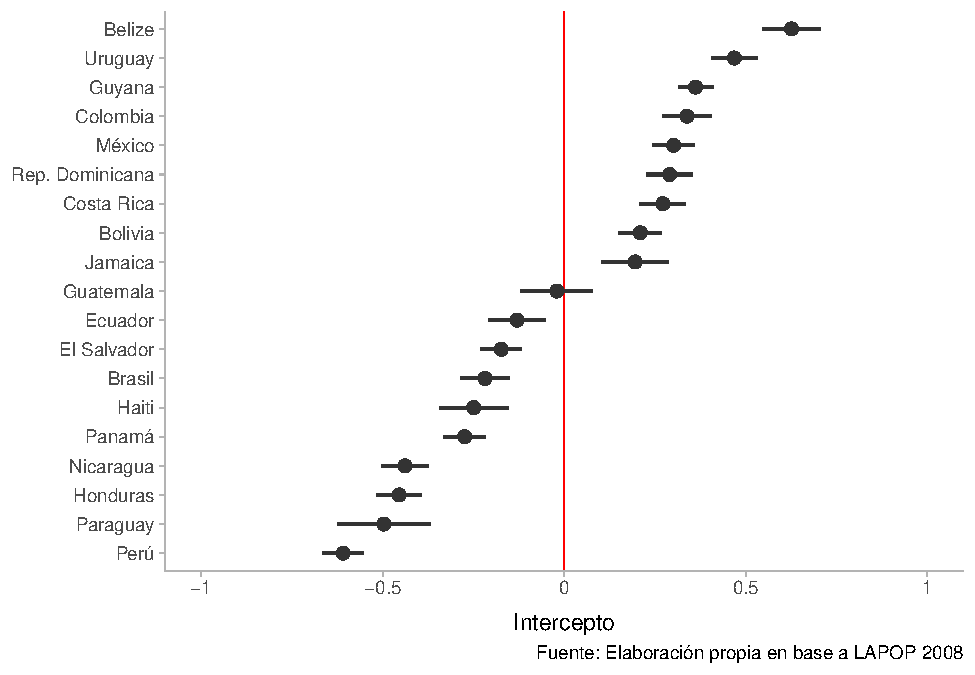
\includegraphics{01-guia_files/figure-latex/fig1-1} 

}

\caption{Interceptos aleatorios por país}\label{fig:fig1}
\end{figure}

\begin{figure}

{\centering 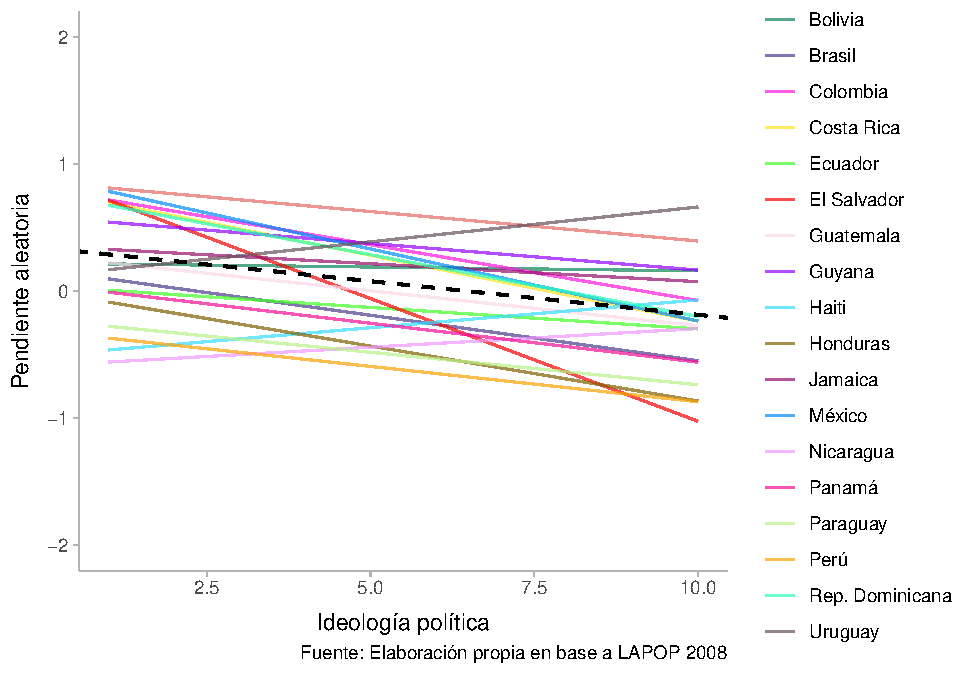
\includegraphics{01-guia_files/figure-latex/fig2-1} 

}

\caption{Pendientes aleatorias de ideología política por país}\label{fig:fig2}
\end{figure}

\begin{figure}

{\centering 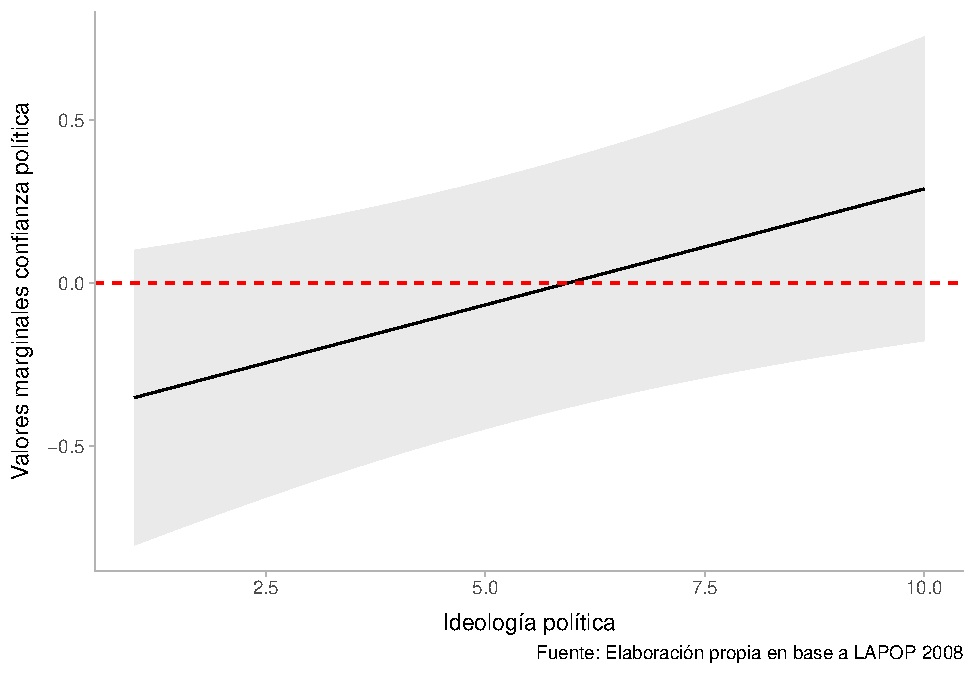
\includegraphics{01-guia_files/figure-latex/fig3-1} 

}

\caption{Valores marginales de ideología moderado por presidencia de izquierda}\label{fig:fig3}
\end{figure}

\pagebreak

\begin{table}[h!]
\begin{center}
\scalebox{0.9}{
\begin{threeparttable}
\begin{tabular}{l c c c}
\toprule
 & Modelo 4 & Modelo 5 & Modelo 6 \\
\midrule
Intercepto                     & $0.41^{***}$  & $0.08$        & $0.61^{*}$    \\
                               & $(0.08)$      & $(0.41)$      & $(0.24)$      \\
Mujer (Ref.= Hombre)           & $-0.02$       & $-0.02$       & $-0.02$       \\
                               & $(0.02)$      & $(0.02)$      & $(0.02)$      \\
Edad                           & $0.00$        & $0.00$        & $0.09^{*}$    \\
                               & $(0.01)$      & $(0.01)$      & $(0.04)$      \\
Nivel educacional (en años)    & $-0.01^{***}$ & $-0.01^{***}$ & $-0.01^{***}$ \\
                               & $(0.00)$      & $(0.00)$      & $(0.00)$      \\
Empleado (Ref.= Desempleado)   & $-0.05^{*}$   & $-0.05^{*}$   & $-0.04^{*}$   \\
                               & $(0.02)$      & $(0.02)$      & $(0.02)$      \\
Casado (Ref.= Otro)            & $0.05^{**}$   & $0.05^{**}$   & $0.05^{**}$   \\
                               & $(0.02)$      & $(0.02)$      & $(0.02)$      \\
Ideología política             & $-0.07^{***}$ & $-0.07^{***}$ & $-0.07^{***}$ \\
                               & $(0.00)$      & $(0.00)$      & $(0.00)$      \\
Participación laboral femenina &               & $0.61$        &               \\
                               &               & $(0.73)$      &               \\
Índice Freedom House           &               &               & $-0.08$       \\
                               &               &               & $(0.09)$      \\
Edad x Índice Freedom House    &               &               & $-0.04^{**}$  \\
                               &               &               & $(0.01)$      \\
\midrule
AIC                            & $52805.69$    & $52805.82$    & $52812.29$    \\
BIC                            & $52899.27$    & $52907.20$    & $52921.47$    \\
-2*log-likelihood              & $-26390.84$   & $-26389.91$   & $-26392.14$   \\
Num. obs                       & $18012$       & $18012$       & $18012$       \\
Num. grupos: Países            & $19$          & $19$          & $19$          \\
Var: Países (Intercepto)       & $0.10$        & $0.11$        & $0.10$        \\
Var: Países Edad               & $0.00$        & $0.00$        & $0.00$        \\
Cov: Países (Intercepto), Edad & $0.00$        & $0.00$        & $0.00$        \\
Var: Residual                  & $1.09$        & $1.09$        & $1.09$        \\
\bottomrule
\end{tabular}
\begin{tablenotes}[flushleft]
\scriptsize{\item Nota: Celdas contienen coeficientes de regresión con errores estándares entre paréntesis. $^{***}p<0.001$; $^{**}p<0.01$; $^{*}p<0.05$ \\ \item Fuente: Elaboración propia en base a LAPOP 2008.}
\end{tablenotes}
\end{threeparttable}
}
\caption{\label{tab:table2} Modelos multinivel para confianza política, edad e índice de democracía del país}
\label{table:coefficients}
\end{center}
\end{table}

Si bien la primera parte del supuesto de sequential unconfoundedness es más plausible de corregir, la segunda no lo es tanto. El sesgo de variable omitida o de heterogeneidad no observada en estudios observacionales es difícil de combatir, ya que generalmente existen variables no observadas postratamiento que pueden confundir el efecto del mediador en la variable de resultado (\protect\hyperlink{ref-acharya_explaining_2016}{Acharya et al., 2016}). Precisamente, esto es lo que Pepinsky et al. (\protect\hyperlink{ref-pepinsky_causation_2024}{2024}) cuestionan en la estrategia de identificación de Homola et al. (\protect\hyperlink{ref-homola_fixed_2024}{2024}), al asumir que no existen confounders intermedios \(Z_i\) no observados que puedan afectar la estimación causal de la distancia a los campos en la intolerancia, lo cual es difícil de sostener.

\begin{table}[!h]

\caption{\label{tab:table3}\label{tab:table3} Estadísticos de bondad de ajuste}
\centering
\begin{tabular}[t]{>{\raggedright\arraybackslash}p{2cm}rrrrrl}
\toprule
\textbf{Modelo} & \textbf{AIC} & \textbf{BIC} & \textbf{Deviance} & \textbf{X2} & \textbf{Df} & \textbf{p-value}\\
\midrule
Modelo 1 & 52822.33 & 52900.32 & 52802.33 &  &  & \\
Modelo 4 & 52750.41 & 52844.00 & 52726.41 & 75.92 & 2 & < 0.001 ***\\
\bottomrule
\end{tabular}
\end{table}

\newpage

\hypertarget{referencias}{%
\section{Referencias}\label{referencias}}

\hypertarget{refs}{}
\begin{CSLReferences}{1}{0}
\leavevmode\vadjust pre{\hypertarget{ref-acharya_explaining_2016}{}}%
Acharya, A., Blackwell, M., \& Sen, M. (2016). Explaining {Causal Findings Without Bias}: {Detecting} and {Assessing Direct Effects}. \emph{American Political Science Review}, \emph{110}(3), 512--529. \url{https://doi.org/10.1017/S0003055416000216}

\leavevmode\vadjust pre{\hypertarget{ref-homola_fixed_2024}{}}%
Homola, J., Pereira, M. M., \& Tavits, M. (2024). Fixed {Effects} and {Post-Treatment Bias} in {Legacy Studies}. \emph{American Political Science Review}, \emph{118}(1), 537--544. \url{https://doi.org/10.1017/S0003055423001351}

\leavevmode\vadjust pre{\hypertarget{ref-pepinsky_causation_2024}{}}%
Pepinsky, T. B., Goodman, S. W., \& Ziller, C. (2024). Causation and {History} in {Legacy Studies}: {A Reply} to {Homola}, {Pereira}, and {Tavits}. \emph{SSRN Electronic Journal}. \url{https://doi.org/10.2139/ssrn.4705690}

\end{CSLReferences}

\pagebreak

\hypertarget{cuxf3digo-de-r}{%
\section{Código de R}\label{cuxf3digo-de-r}}

\begin{Shaded}
\begin{Highlighting}[]
\NormalTok{knitr}\SpecialCharTok{::}\NormalTok{opts\_chunk}\SpecialCharTok{$}\FunctionTok{set}\NormalTok{(}\AttributeTok{echo =}\NormalTok{ F,}
                      \AttributeTok{warning =}\NormalTok{ F,}
                      \AttributeTok{error =}\NormalTok{ F, }
                      \AttributeTok{message =}\NormalTok{ F) }
\ControlFlowTok{if}\NormalTok{ (}\SpecialCharTok{!} \FunctionTok{require}\NormalTok{(}\StringTok{"pacman"}\NormalTok{)) }\FunctionTok{install.packages}\NormalTok{(}\StringTok{"pacman"}\NormalTok{)}

\NormalTok{pacman}\SpecialCharTok{::}\FunctionTok{p\_load}\NormalTok{(tidyverse, }
\NormalTok{               sjmisc, }
\NormalTok{               sjPlot, }
\NormalTok{               lme4, }
\NormalTok{               easystats, }
\NormalTok{               influence.ME, }
\NormalTok{               performance,}
\NormalTok{               broom.mixed, }
\NormalTok{               here,}
\NormalTok{               texreg, }
\NormalTok{               ggeffects,}
\NormalTok{               marginaleffects,}
\NormalTok{               naniar,}
\NormalTok{               ggdist,}
\NormalTok{               Polychrome,}
\NormalTok{               misty,}
\NormalTok{               kableExtra)}

\FunctionTok{options}\NormalTok{(}\AttributeTok{scipen=}\DecValTok{999}\NormalTok{)}
\FunctionTok{rm}\NormalTok{(}\AttributeTok{list =} \FunctionTok{ls}\NormalTok{())}

\NormalTok{miles }\OtherTok{\textless{}{-}} \ControlFlowTok{function}\NormalTok{(x) \{}
  \FunctionTok{format}\NormalTok{(}\FunctionTok{round}\NormalTok{(}\FunctionTok{as.numeric}\NormalTok{(x),}\DecValTok{0}\NormalTok{), }\AttributeTok{big.mark =} \StringTok{"."}\NormalTok{)}
\NormalTok{\}}

\NormalTok{decimales }\OtherTok{\textless{}{-}} \ControlFlowTok{function}\NormalTok{(x) \{}
  \FunctionTok{format}\NormalTok{(}\FunctionTok{round}\NormalTok{(}\FunctionTok{as.numeric}\NormalTok{(x), }\DecValTok{2}\NormalTok{), }\AttributeTok{decimal.mark =} \StringTok{","}\NormalTok{)}
\NormalTok{\}}

\CommentTok{\# set theme}

\FunctionTok{theme\_set}\NormalTok{(}\FunctionTok{theme\_ggdist}\NormalTok{())}

\FunctionTok{options}\NormalTok{(}\AttributeTok{knitr.kable.NA =} \StringTok{""}\NormalTok{)}
\FunctionTok{options}\NormalTok{(}\AttributeTok{knitr.table.format=}\StringTok{"latex"}\NormalTok{)}

\FunctionTok{load}\NormalTok{(}\AttributeTok{file =} \FunctionTok{here}\NormalTok{(}\StringTok{"input/data/morgan2013.RData"}\NormalTok{))}

\FunctionTok{names}\NormalTok{(morgan2013)}
\FunctionTok{glimpse}\NormalTok{(morgan2013)}

\CommentTok{\# seleccionar {-}{-}{-}{-}}

\NormalTok{db }\OtherTok{\textless{}{-}}\NormalTok{ morgan2013 }\SpecialCharTok{\%\textgreater{}\%} 
  \FunctionTok{select}\NormalTok{(country, ID, trustgov, }\AttributeTok{sex =}\NormalTok{ female, age, educ, employed, married,}
\NormalTok{         race, }\AttributeTok{ideology =}\NormalTok{ left, leftpres, FLP, fhouse) }\SpecialCharTok{\%\textgreater{}\%} 
\NormalTok{  sjlabelled}\SpecialCharTok{::}\FunctionTok{remove\_all\_labels}\NormalTok{() }\SpecialCharTok{\%\textgreater{}\%} 
\NormalTok{  janitor}\SpecialCharTok{::}\FunctionTok{clean\_names}\NormalTok{() }\SpecialCharTok{\%\textgreater{}\%} 
  \FunctionTok{as\_tibble}\NormalTok{()}
 
\CommentTok{\# filtrar: no {-}{-}{-}{-}{-} }

\CommentTok{\# recodificar y transformar {-}{-}{-}{-}}

\CommentTok{\# trust}
\NormalTok{sjmisc}\SpecialCharTok{::}\FunctionTok{descr}\NormalTok{(db}\SpecialCharTok{$}\NormalTok{in\_trust)}

\CommentTok{\# sexo}
\FunctionTok{frq}\NormalTok{(db}\SpecialCharTok{$}\NormalTok{sex)}

\NormalTok{db}\SpecialCharTok{$}\NormalTok{sex }\OtherTok{\textless{}{-}}\NormalTok{ car}\SpecialCharTok{::}\FunctionTok{recode}\NormalTok{(db}\SpecialCharTok{$}\NormalTok{sex, }
                      \AttributeTok{recodes=} \FunctionTok{c}\NormalTok{(}\StringTok{"0=\textquotesingle{}Hombre\textquotesingle{};1=\textquotesingle{}Mujer\textquotesingle{}"}\NormalTok{),}
                      \AttributeTok{levels =} \FunctionTok{c}\NormalTok{(}\StringTok{"Hombre"}\NormalTok{,}\StringTok{"Mujer"}\NormalTok{),}
                      \AttributeTok{as.factor =}\NormalTok{ T)}

\CommentTok{\# edad}
\NormalTok{sjmisc}\SpecialCharTok{::}\FunctionTok{descr}\NormalTok{(db}\SpecialCharTok{$}\NormalTok{age)}
\FunctionTok{frq}\NormalTok{(db}\SpecialCharTok{$}\NormalTok{age)}

\NormalTok{db}\SpecialCharTok{$}\NormalTok{age\_f }\OtherTok{\textless{}{-}}\NormalTok{ car}\SpecialCharTok{::}\FunctionTok{recode}\NormalTok{(db}\SpecialCharTok{$}\NormalTok{age, }
                      \AttributeTok{recodes =} \FunctionTok{c}\NormalTok{(}\StringTok{"1=\textquotesingle{}Tramo 1\textquotesingle{};}
\StringTok{                                  2=\textquotesingle{}Tramo 2\textquotesingle{};}
\StringTok{                                  3=\textquotesingle{}Tramo 3\textquotesingle{};}
\StringTok{                                  4=\textquotesingle{}Tramo 4\textquotesingle{};}
\StringTok{                                  5=\textquotesingle{}Tramo 5\textquotesingle{};}
\StringTok{                                  6=\textquotesingle{}Tramo 6\textquotesingle{}"}\NormalTok{),}
                      \AttributeTok{levels =} \FunctionTok{c}\NormalTok{(}\StringTok{"Tramo 1"}\NormalTok{,}
                                 \StringTok{"Tramo 2"}\NormalTok{,   }
                                 \StringTok{"Tramo 3"}\NormalTok{,   }
                                 \StringTok{"Tramo 4"}\NormalTok{,    }
                                 \StringTok{"Tramo 5"}\NormalTok{,   }
                                 \StringTok{"Tramo 6"}\NormalTok{),}
                      \AttributeTok{as.factor =}\NormalTok{ T}
\NormalTok{)}

\CommentTok{\# educ}
\NormalTok{sjmisc}\SpecialCharTok{::}\FunctionTok{descr}\NormalTok{(db}\SpecialCharTok{$}\NormalTok{educ)}

\CommentTok{\# employed}
\FunctionTok{frq}\NormalTok{(db}\SpecialCharTok{$}\NormalTok{employed)}

\NormalTok{db}\SpecialCharTok{$}\NormalTok{employed }\OtherTok{\textless{}{-}}\NormalTok{ car}\SpecialCharTok{::}\FunctionTok{recode}\NormalTok{(db}\SpecialCharTok{$}\NormalTok{employed, }
                      \AttributeTok{recodes=} \FunctionTok{c}\NormalTok{(}\StringTok{"0=\textquotesingle{}Desempleado\textquotesingle{};1=\textquotesingle{}Empleado\textquotesingle{}"}\NormalTok{),}
                      \AttributeTok{levels =} \FunctionTok{c}\NormalTok{(}\StringTok{"Desempleado"}\NormalTok{,}\StringTok{"Empleado"}\NormalTok{),}
                      \AttributeTok{as.factor =}\NormalTok{ T)}
\CommentTok{\# married}
\FunctionTok{frq}\NormalTok{(db}\SpecialCharTok{$}\NormalTok{married)}

\NormalTok{db}\SpecialCharTok{$}\NormalTok{married }\OtherTok{\textless{}{-}}\NormalTok{ car}\SpecialCharTok{::}\FunctionTok{recode}\NormalTok{(db}\SpecialCharTok{$}\NormalTok{married, }
                      \AttributeTok{recodes=} \FunctionTok{c}\NormalTok{(}\StringTok{"0=\textquotesingle{}No\textquotesingle{};1=\textquotesingle{}Sí\textquotesingle{}"}\NormalTok{),}
                      \AttributeTok{levels =} \FunctionTok{c}\NormalTok{(}\StringTok{"No"}\NormalTok{,}\StringTok{"Sí"}\NormalTok{),}
                      \AttributeTok{as.factor =}\NormalTok{ T)}

\CommentTok{\# race}
\FunctionTok{frq}\NormalTok{(db}\SpecialCharTok{$}\NormalTok{race)}

\NormalTok{db}\SpecialCharTok{$}\NormalTok{race }\OtherTok{\textless{}{-}}\NormalTok{ car}\SpecialCharTok{::}\FunctionTok{recode}\NormalTok{(db}\SpecialCharTok{$}\NormalTok{race, }
                      \AttributeTok{recodes=} \FunctionTok{c}\NormalTok{(}\StringTok{"0=\textquotesingle{}Otro\textquotesingle{};1=\textquotesingle{}Blanco\textquotesingle{}"}\NormalTok{),}
                      \AttributeTok{levels =} \FunctionTok{c}\NormalTok{(}\StringTok{"Otro"}\NormalTok{,}\StringTok{"Blanco"}\NormalTok{),}
                      \AttributeTok{as.factor =}\NormalTok{ T)}

\CommentTok{\# ideology}
\FunctionTok{frq}\NormalTok{(db}\SpecialCharTok{$}\NormalTok{ideology)}

\CommentTok{\# left}
\FunctionTok{frq}\NormalTok{(db}\SpecialCharTok{$}\NormalTok{leftpres)}

\NormalTok{db}\SpecialCharTok{$}\NormalTok{leftpres }\OtherTok{\textless{}{-}}\NormalTok{ car}\SpecialCharTok{::}\FunctionTok{recode}\NormalTok{(db}\SpecialCharTok{$}\NormalTok{leftpres, }
                      \AttributeTok{recodes=} \FunctionTok{c}\NormalTok{(}\StringTok{"0=\textquotesingle{}No\textquotesingle{};1=\textquotesingle{}Sí\textquotesingle{}"}\NormalTok{),}
                      \AttributeTok{levels =} \FunctionTok{c}\NormalTok{(}\StringTok{"No"}\NormalTok{,}\StringTok{"Sí"}\NormalTok{),}
                      \AttributeTok{as.factor =}\NormalTok{ T)}


\CommentTok{\# flp}
\NormalTok{sjmisc}\SpecialCharTok{::}\FunctionTok{descr}\NormalTok{(db}\SpecialCharTok{$}\NormalTok{flp)}

\CommentTok{\# fhouse}
\NormalTok{sjmisc}\SpecialCharTok{::}\FunctionTok{descr}\NormalTok{(db}\SpecialCharTok{$}\NormalTok{fhouse)}

\CommentTok{\# id}
\NormalTok{sjmisc}\SpecialCharTok{::}\FunctionTok{descr}\NormalTok{(db}\SpecialCharTok{$}\NormalTok{id)}

\CommentTok{\# country}
\FunctionTok{frq}\NormalTok{(db}\SpecialCharTok{$}\NormalTok{country)}

\CommentTok{\# casos perdidos {-}{-}{-}{-}{-}}

\FunctionTok{colSums}\NormalTok{(}\FunctionTok{is.na}\NormalTok{(db))}

\FunctionTok{n\_miss}\NormalTok{(db)}

\FunctionTok{prop\_miss}\NormalTok{(db)}\SpecialCharTok{*}\DecValTok{100}

\FunctionTok{miss\_var\_summary}\NormalTok{(db)}

\FunctionTok{miss\_var\_table}\NormalTok{(db)}

\FunctionTok{vis\_miss}\NormalTok{(db) }\SpecialCharTok{+} \FunctionTok{theme}\NormalTok{(}\AttributeTok{axis.text.x =} \FunctionTok{element\_text}\NormalTok{(}\AttributeTok{angle=}\DecValTok{80}\NormalTok{))}

\NormalTok{db }\OtherTok{\textless{}{-}} \FunctionTok{na.omit}\NormalTok{(db)}

\CommentTok{\# Null model}
\NormalTok{model\_0 }\OtherTok{\textless{}{-}} \FunctionTok{lmer}\NormalTok{(in\_trust }\SpecialCharTok{\textasciitilde{}} \DecValTok{1} \SpecialCharTok{+}\NormalTok{ (}\DecValTok{1} \SpecialCharTok{|}\NormalTok{ country), }
                \AttributeTok{data =}\NormalTok{ db, }\AttributeTok{REML =}\NormalTok{ T)}

\NormalTok{performance}\SpecialCharTok{::}\FunctionTok{icc}\NormalTok{(model\_0, }\AttributeTok{by\_group =}\NormalTok{ T)}
\DocumentationTok{\#\# ICC Country = 0.11}

\CommentTok{\# Influence test}
\NormalTok{inf\_m0 }\OtherTok{\textless{}{-}} \FunctionTok{influence}\NormalTok{(model\_0, }\AttributeTok{group =} \StringTok{"country"}\NormalTok{)}

\CommentTok{\# D cook}
\FunctionTok{cooks.distance}\NormalTok{(inf\_m0, }\AttributeTok{parameters =} \DecValTok{1}\NormalTok{, }\AttributeTok{sort =}\NormalTok{ T) }\CommentTok{\# cut point is 4/19 }

\NormalTok{n\_country }\OtherTok{\textless{}{-}} \FunctionTok{length}\NormalTok{(}\FunctionTok{unique}\NormalTok{(db}\SpecialCharTok{$}\NormalTok{country))}

\FunctionTok{plot}\NormalTok{(inf\_m0, }\AttributeTok{which=}\StringTok{"cook"}\NormalTok{,}
     \AttributeTok{cutoff=}\NormalTok{(}\DecValTok{4}\SpecialCharTok{/}\NormalTok{n\_country), }\AttributeTok{sort=}\ConstantTok{TRUE}\NormalTok{,}
     \AttributeTok{xlab=}\StringTok{"Distancia de Cook"}\NormalTok{,}
     \AttributeTok{ylab=}\StringTok{"País"}\NormalTok{, }\AttributeTok{width=}\DecValTok{60}\NormalTok{, }\AttributeTok{height=}\DecValTok{40}\NormalTok{)}

\CommentTok{\# no obs influyentes}

\CommentTok{\# Modelo 1: Indicadores N1}
\NormalTok{model\_1 }\OtherTok{\textless{}{-}} \FunctionTok{lmer}\NormalTok{(in\_trust }\SpecialCharTok{\textasciitilde{}} \DecValTok{1} \SpecialCharTok{+}\NormalTok{ sex }\SpecialCharTok{+}\NormalTok{ age }\SpecialCharTok{+}\NormalTok{ educ }\SpecialCharTok{+}\NormalTok{ employed }\SpecialCharTok{+}\NormalTok{ married }\SpecialCharTok{+}
\NormalTok{                race }\SpecialCharTok{+}\NormalTok{ ideology }\SpecialCharTok{+}\NormalTok{ (}\DecValTok{1} \SpecialCharTok{|}\NormalTok{ country),}
                \AttributeTok{data =}\NormalTok{ db, }
                \AttributeTok{REML =}\NormalTok{ T)}

\CommentTok{\# Modelo 2: Pendiente aleatoria ideology}
\NormalTok{model\_2 }\OtherTok{\textless{}{-}} \FunctionTok{lmer}\NormalTok{(in\_trust }\SpecialCharTok{\textasciitilde{}} \DecValTok{1} \SpecialCharTok{+}\NormalTok{ sex }\SpecialCharTok{+}\NormalTok{ age }\SpecialCharTok{+}\NormalTok{ educ }\SpecialCharTok{+}\NormalTok{ employed }\SpecialCharTok{+}\NormalTok{ married }\SpecialCharTok{+}
\NormalTok{                race }\SpecialCharTok{+}\NormalTok{ ideology }\SpecialCharTok{+}\NormalTok{ (}\DecValTok{1} \SpecialCharTok{+}\NormalTok{ ideology}\SpecialCharTok{|}\NormalTok{ country),}
                \AttributeTok{data =}\NormalTok{ db, }
                \AttributeTok{REML =}\NormalTok{ T)}

\CommentTok{\# Modelo 3: Interaccion ideology y leftpres}
\NormalTok{model\_3 }\OtherTok{\textless{}{-}} \FunctionTok{lmer}\NormalTok{(in\_trust }\SpecialCharTok{\textasciitilde{}} \DecValTok{1} \SpecialCharTok{+}\NormalTok{ sex }\SpecialCharTok{+}\NormalTok{ age }\SpecialCharTok{+}\NormalTok{ educ }\SpecialCharTok{+}\NormalTok{ employed }\SpecialCharTok{+}\NormalTok{ married }\SpecialCharTok{+}
\NormalTok{                race }\SpecialCharTok{+}\NormalTok{ ideology }\SpecialCharTok{+}\NormalTok{ leftpres }\SpecialCharTok{+}\NormalTok{ ideology}\SpecialCharTok{*}\NormalTok{leftpres }\SpecialCharTok{+} 
\NormalTok{                (}\DecValTok{1} \SpecialCharTok{+}\NormalTok{ ideology}\SpecialCharTok{|}\NormalTok{ country),}
                \AttributeTok{data =}\NormalTok{ db, }
                \AttributeTok{REML =}\NormalTok{ T)}

\CommentTok{\# Modelo 4: Pendiente aleatoria edad}
\NormalTok{model\_4 }\OtherTok{\textless{}{-}} \FunctionTok{lmer}\NormalTok{(in\_trust }\SpecialCharTok{\textasciitilde{}} \DecValTok{1} \SpecialCharTok{+}\NormalTok{ sex }\SpecialCharTok{+}\NormalTok{ age }\SpecialCharTok{+}\NormalTok{ educ }\SpecialCharTok{+}\NormalTok{ employed }\SpecialCharTok{+}\NormalTok{ married }\SpecialCharTok{+}
\NormalTok{                race }\SpecialCharTok{+}\NormalTok{ ideology }\SpecialCharTok{+}\NormalTok{ (}\DecValTok{1} \SpecialCharTok{+}\NormalTok{ age}\SpecialCharTok{|}\NormalTok{ country),}
                \AttributeTok{data =}\NormalTok{ db, }
                \AttributeTok{REML =}\NormalTok{ T)}

\CommentTok{\# Modelo 5: Pendiente aleatoria edad + flp}
\NormalTok{model\_5 }\OtherTok{\textless{}{-}} \FunctionTok{lmer}\NormalTok{(in\_trust }\SpecialCharTok{\textasciitilde{}} \DecValTok{1} \SpecialCharTok{+}\NormalTok{ sex }\SpecialCharTok{+}\NormalTok{ age }\SpecialCharTok{+}\NormalTok{ educ }\SpecialCharTok{+}\NormalTok{ employed }\SpecialCharTok{+}\NormalTok{ married }\SpecialCharTok{+}
\NormalTok{                race }\SpecialCharTok{+}\NormalTok{ ideology }\SpecialCharTok{+}\NormalTok{ flp }\SpecialCharTok{+}\NormalTok{ (}\DecValTok{1} \SpecialCharTok{+}\NormalTok{ age}\SpecialCharTok{|}\NormalTok{ country),}
                \AttributeTok{data =}\NormalTok{ db, }
                \AttributeTok{REML =}\NormalTok{ T)}

\CommentTok{\# Modelo 6: Pendiente aleatoria edad + flp}
\NormalTok{model\_6 }\OtherTok{\textless{}{-}} \FunctionTok{lmer}\NormalTok{(in\_trust }\SpecialCharTok{\textasciitilde{}} \DecValTok{1} \SpecialCharTok{+}\NormalTok{ sex }\SpecialCharTok{+}\NormalTok{ age }\SpecialCharTok{+}\NormalTok{ educ }\SpecialCharTok{+}\NormalTok{ employed }\SpecialCharTok{+}\NormalTok{ married }\SpecialCharTok{+}
\NormalTok{                race }\SpecialCharTok{+}\NormalTok{ ideology }\SpecialCharTok{+}\NormalTok{ age}\SpecialCharTok{*}\NormalTok{fhouse }\SpecialCharTok{+}\NormalTok{ (}\DecValTok{1} \SpecialCharTok{+}\NormalTok{ age}\SpecialCharTok{|}\NormalTok{ country),}
                \AttributeTok{data =}\NormalTok{ db, }
                \AttributeTok{REML =}\NormalTok{ T)}


\NormalTok{ccoef }\OtherTok{\textless{}{-}} \FunctionTok{list}\NormalTok{(}
  \StringTok{"(Intercept)"} \OtherTok{=} \StringTok{"Intercepto"}\NormalTok{,}
  \AttributeTok{sexMujer =} \StringTok{"Mujer (Ref.= Hombre)"}\NormalTok{,}
  \AttributeTok{age =} \StringTok{"Edad"}\NormalTok{,}
  \AttributeTok{educ =} \StringTok{"Nivel educacional (en años)"}\NormalTok{,}
  \AttributeTok{employedEmpleado =} \StringTok{"Empleado (Ref.= Desempleado)"}\NormalTok{,}
\NormalTok{  marriedSí }\OtherTok{=} \StringTok{"Casado (Ref.= Otro)"}\NormalTok{,}
  \AttributeTok{race =} \StringTok{"Blanco (Ref.= Otro)"}\NormalTok{,}
  \AttributeTok{ideology =} \StringTok{"Ideología política"}\NormalTok{,}
\NormalTok{  leftpresSí }\OtherTok{=} \StringTok{"Presidencia Izquierda (Ref. = Otra)"}\NormalTok{,}
  \StringTok{"ideology:leftpresSí"} \OtherTok{=} \StringTok{"Ideología política x Presidencia Izquierda (Ref. = Otra)"}\NormalTok{)}


\NormalTok{texreg}\SpecialCharTok{::}\FunctionTok{texreg}\NormalTok{(}\FunctionTok{list}\NormalTok{(model\_1, model\_2, model\_3),}
               \AttributeTok{custom.model.names =} \FunctionTok{c}\NormalTok{(}\StringTok{"Modelo 1"}\NormalTok{,}
                                      \StringTok{"Modelo 2"}\NormalTok{,}
                                      \StringTok{"Modelo 3"}\NormalTok{),}
               \AttributeTok{caption =} \FunctionTok{paste}\NormalTok{(}\StringTok{"(}\SpecialCharTok{\textbackslash{}\textbackslash{}}\StringTok{\#tab:table1)"}\NormalTok{,}\StringTok{"Modelos multinivel para confianza política, ideología política y países con presidencia de izquierda"}\NormalTok{),}
               \AttributeTok{stars =} \FunctionTok{c}\NormalTok{(}\FloatTok{0.05}\NormalTok{, }\FloatTok{0.01}\NormalTok{, }\FloatTok{0.001}\NormalTok{),}
               \AttributeTok{custom.coef.map =}\NormalTok{ ccoef,}
               \AttributeTok{custom.note =} \StringTok{"}\SpecialCharTok{\textbackslash{}\textbackslash{}}\StringTok{item Nota: Celdas contienen coeficientes de regresión con errores estándares entre paréntesis. \%stars }\SpecialCharTok{\textbackslash{}\textbackslash{}\textbackslash{}\textbackslash{}}\StringTok{ }\SpecialCharTok{\textbackslash{}\textbackslash{}}\StringTok{item Fuente: Elaboración propia en base a LAPOP 2008."}\NormalTok{,}
               \AttributeTok{threeparttable =}\NormalTok{ T,}
               \AttributeTok{leading.zero =}\NormalTok{ T,}
               \AttributeTok{float.pos =} \StringTok{"h!"}\NormalTok{,}
               \AttributeTok{use.packages =}\NormalTok{ F,}
               \AttributeTok{booktabs =} \ConstantTok{TRUE}\NormalTok{,}
               \AttributeTok{scalebox =} \FloatTok{0.9}\NormalTok{,}
               \AttributeTok{custom.gof.names =} \FunctionTok{c}\NormalTok{(}\StringTok{"AIC"}\NormalTok{, }
                                    \StringTok{"BIC"}\NormalTok{, }
                                    \StringTok{"{-}2*log{-}likelihood"}\NormalTok{, }
                                    \StringTok{"Num. obs"}\NormalTok{, }
                                    \StringTok{"Num. grupos: Países"}\NormalTok{,}
                                    \StringTok{"Var: Países (Intercepto)"}\NormalTok{,}
                                    \StringTok{"Var: Residual"}\NormalTok{,}
                                    \StringTok{"Var: Países Ideología"}\NormalTok{,}
                                    \StringTok{"Cov: Países (Intercepto), Ideología"}
\NormalTok{                                    ))}
\NormalTok{sjPlot}\SpecialCharTok{::}\FunctionTok{plot\_model}\NormalTok{(model\_1, }
                   \AttributeTok{type =} \StringTok{"re"}\NormalTok{, }
                   \AttributeTok{vline.color =} \StringTok{"red"}\NormalTok{,}
                   \AttributeTok{grid =}\NormalTok{ F, }
                   \AttributeTok{sort.est =} \StringTok{"sort.all"}\NormalTok{, }
                   \AttributeTok{ci.lvl =}\NormalTok{ .}\DecValTok{95}\NormalTok{, }
                   \AttributeTok{colors =} \StringTok{"grey20"}\NormalTok{) }\SpecialCharTok{+}
  \FunctionTok{labs}\NormalTok{(}\AttributeTok{title =} \ConstantTok{NULL}\NormalTok{,}
       \AttributeTok{y =} \StringTok{"Intercepto"}\NormalTok{,}
       \AttributeTok{caption =} \StringTok{"Fuente: Elaboración propia en base a LAPOP 2008"}\NormalTok{)}\SpecialCharTok{+}
  \FunctionTok{theme\_ggdist}\NormalTok{()}


\NormalTok{stats\_m2 }\OtherTok{\textless{}{-}}\NormalTok{ broom.mixed}\SpecialCharTok{::}\FunctionTok{tidy}\NormalTok{(model\_2)}

\NormalTok{ideology\_rang }\OtherTok{\textless{}{-}} \FunctionTok{seq}\NormalTok{(}\DecValTok{1}\SpecialCharTok{:}\DecValTok{10}\NormalTok{)}
\NormalTok{in\_trust2 }\OtherTok{\textless{}{-}} \FunctionTok{as.data.frame}\NormalTok{(}\FunctionTok{sapply}\NormalTok{(ideology\_rang,}\ControlFlowTok{function}\NormalTok{(x)}\FunctionTok{fixef}\NormalTok{(model\_2)[}\StringTok{"(Intercept)"}\NormalTok{] }\SpecialCharTok{+} 
                                    \FunctionTok{fixef}\NormalTok{(model\_2)[}\StringTok{"sexMujer"}\NormalTok{]}\SpecialCharTok{*}\DecValTok{0} \SpecialCharTok{+}
                                    \FunctionTok{fixef}\NormalTok{(model\_2)[}\StringTok{"age"}\NormalTok{]}\SpecialCharTok{*}\FloatTok{2.74} \SpecialCharTok{+}
                                    \FunctionTok{fixef}\NormalTok{(model\_2)[}\StringTok{"educ"}\NormalTok{]}\SpecialCharTok{*}\FloatTok{9.23} \SpecialCharTok{+}
                                    \FunctionTok{fixef}\NormalTok{(model\_2)[}\StringTok{"employedEmpleado"}\NormalTok{]}\SpecialCharTok{*}\DecValTok{1} \SpecialCharTok{+}
                                    \FunctionTok{fixef}\NormalTok{(model\_2)[}\StringTok{"marriedSí"}\NormalTok{]}\SpecialCharTok{*}\DecValTok{1} \SpecialCharTok{+}
                                    \FunctionTok{fixef}\NormalTok{(model\_2)[}\StringTok{"raceBlanco"}\NormalTok{]}\SpecialCharTok{*}\DecValTok{0} \SpecialCharTok{+}
                                    \FunctionTok{fixef}\NormalTok{(model\_2)[}\StringTok{"ideology"}\NormalTok{]}\SpecialCharTok{*}\NormalTok{x }\SpecialCharTok{+}
                                    \FunctionTok{ranef}\NormalTok{(model\_2)}\SpecialCharTok{$}\NormalTok{country[,}\DecValTok{1}\NormalTok{] }\SpecialCharTok{+}
                                    \FunctionTok{ranef}\NormalTok{(model\_2)}\SpecialCharTok{$}\NormalTok{country[,}\DecValTok{2}\NormalTok{]}\SpecialCharTok{*}\NormalTok{x))}

\NormalTok{in\_trust2}\SpecialCharTok{$}\NormalTok{country }\OtherTok{\textless{}{-}} \FunctionTok{seq}\NormalTok{(}\DecValTok{1}\SpecialCharTok{:}\DecValTok{19}\NormalTok{)}
\NormalTok{in\_trust2 }\OtherTok{\textless{}{-}} \FunctionTok{reshape}\NormalTok{(in\_trust2,}
                     \AttributeTok{direction =} \StringTok{"long"}\NormalTok{, }\CommentTok{\#formato long}
                     \AttributeTok{v.names =} \StringTok{"pred"}\NormalTok{,}
                     \AttributeTok{varying =} \FunctionTok{list}\NormalTok{(}\FunctionTok{names}\NormalTok{(in\_trust2)[}\DecValTok{1}\SpecialCharTok{:}\DecValTok{10}\NormalTok{]),}
                     \AttributeTok{idvar =} \FunctionTok{c}\NormalTok{(}\StringTok{"country"}\NormalTok{),}
                     \AttributeTok{timevar =} \StringTok{"ideology"}\NormalTok{)}

\NormalTok{colores }\OtherTok{\textless{}{-}} \FunctionTok{setNames}\NormalTok{(}\FunctionTok{createPalette}\NormalTok{(}\DecValTok{19}\NormalTok{, }\FunctionTok{c}\NormalTok{(}\StringTok{"\#E16462"}\NormalTok{, }\StringTok{"\#177b4b"}\NormalTok{, }\StringTok{"\#0D0887"}\NormalTok{)), }\FunctionTok{levels}\NormalTok{(db}\SpecialCharTok{$}\NormalTok{country))}


\NormalTok{in\_trust2 }\SpecialCharTok{\%\textgreater{}\%} 
  \FunctionTok{mutate}\NormalTok{(}\AttributeTok{country =} \FunctionTok{factor}\NormalTok{(country, }
                          \AttributeTok{levels =} \DecValTok{1}\SpecialCharTok{:}\DecValTok{19}\NormalTok{,              }
                          \AttributeTok{labels =} \FunctionTok{levels}\NormalTok{(db}\SpecialCharTok{$}\NormalTok{country))) }\SpecialCharTok{\%\textgreater{}\%} 
  \FunctionTok{ggplot}\NormalTok{(}\FunctionTok{aes}\NormalTok{(}\AttributeTok{x =}\NormalTok{ ideology, }\AttributeTok{y =}\NormalTok{ pred, }\AttributeTok{group =}\NormalTok{ country, }\AttributeTok{color =}\NormalTok{ country)) }\SpecialCharTok{+}
  \FunctionTok{geom\_line}\NormalTok{(}\AttributeTok{alpha =} \FloatTok{0.7}\NormalTok{) }\SpecialCharTok{+} 
  \FunctionTok{ylim}\NormalTok{(}\SpecialCharTok{{-}}\DecValTok{2}\NormalTok{,}\DecValTok{2}\NormalTok{) }\SpecialCharTok{+}
  \FunctionTok{geom\_abline}\NormalTok{(}\AttributeTok{intercept =}\NormalTok{ stats\_m2}\SpecialCharTok{$}\NormalTok{estimate[stats\_m2}\SpecialCharTok{$}\NormalTok{term }\SpecialCharTok{==} \StringTok{"(Intercept)"}\NormalTok{],}
              \AttributeTok{slope =}\NormalTok{ stats\_m2}\SpecialCharTok{$}\NormalTok{estimate[stats\_m2}\SpecialCharTok{$}\NormalTok{term }\SpecialCharTok{==} \StringTok{"ideology"}\NormalTok{],}
              \AttributeTok{color =} \StringTok{"black"}\NormalTok{,}
              \AttributeTok{linetype =} \StringTok{"dashed"}\NormalTok{,}
              \AttributeTok{linewidth =} \FloatTok{0.7}\NormalTok{) }\SpecialCharTok{+}
  \FunctionTok{scale\_color\_manual}\NormalTok{(}\AttributeTok{values =}\NormalTok{ colores) }\SpecialCharTok{+}
  \FunctionTok{labs}\NormalTok{(}\AttributeTok{y =} \StringTok{"Pendiente aleatoria"}\NormalTok{,}
       \AttributeTok{x =} \StringTok{"Ideología política"}\NormalTok{,}
       \AttributeTok{color =} \StringTok{"País"}\NormalTok{,}
       \AttributeTok{caption =} \StringTok{"Fuente: Elaboración propia en base a LAPOP 2008"}\NormalTok{) }


\CommentTok{\# manual}

\NormalTok{varcomp\_0}\OtherTok{=}\FunctionTok{as.data.frame}\NormalTok{(}\FunctionTok{VarCorr}\NormalTok{(model\_0))}
\NormalTok{tau00\_0}\OtherTok{=}\NormalTok{varcomp\_0[}\DecValTok{1}\NormalTok{,}\DecValTok{4}\NormalTok{]}
\NormalTok{sigma2\_0}\OtherTok{=}\NormalTok{varcomp\_0[}\DecValTok{2}\NormalTok{,}\DecValTok{4}\NormalTok{]}

\NormalTok{varcomp\_1}\OtherTok{=}\FunctionTok{as.data.frame}\NormalTok{(}\FunctionTok{VarCorr}\NormalTok{(model\_1))}
\NormalTok{tau00\_1}\OtherTok{=}\NormalTok{varcomp\_1[}\DecValTok{1}\NormalTok{,}\DecValTok{4}\NormalTok{]}
\NormalTok{sigma2\_1}\OtherTok{=}\NormalTok{varcomp\_1[}\DecValTok{2}\NormalTok{,}\DecValTok{4}\NormalTok{]}

\NormalTok{R2\_1\_L1}\OtherTok{=}\NormalTok{(sigma2\_0}\SpecialCharTok{{-}}\NormalTok{sigma2\_1)}\SpecialCharTok{/}\NormalTok{sigma2\_0}
\NormalTok{R2\_1\_L1}

\NormalTok{R2\_2\_L1}\OtherTok{=}\NormalTok{(tau00\_0}\SpecialCharTok{{-}}\NormalTok{tau00\_1)}\SpecialCharTok{/}\NormalTok{tau00\_0}
\NormalTok{R2\_2\_L1}

\CommentTok{\# misty}
\NormalTok{db\_n }\OtherTok{\textless{}{-}}\NormalTok{ db }\SpecialCharTok{\%\textgreater{}\%} 
  \FunctionTok{mutate}\NormalTok{(}
    \FunctionTok{across}\NormalTok{(}\AttributeTok{.cols =} \FunctionTok{c}\NormalTok{(sex, age, employed, married, race),}
           \AttributeTok{.fns =} \SpecialCharTok{\textasciitilde{}} \FunctionTok{as.numeric}\NormalTok{(.))}
\NormalTok{  )}
 

\NormalTok{model\_1\_n }\OtherTok{\textless{}{-}} \FunctionTok{lmer}\NormalTok{(in\_trust }\SpecialCharTok{\textasciitilde{}} \DecValTok{1} \SpecialCharTok{+}\NormalTok{ sex }\SpecialCharTok{+}\NormalTok{ age }\SpecialCharTok{+}\NormalTok{ educ }\SpecialCharTok{+}\NormalTok{ employed }\SpecialCharTok{+}\NormalTok{ married }\SpecialCharTok{+}
\NormalTok{                race }\SpecialCharTok{+}\NormalTok{ ideology }\SpecialCharTok{+}\NormalTok{ (}\DecValTok{1} \SpecialCharTok{|}\NormalTok{ country),}
                \AttributeTok{data =}\NormalTok{ db\_n, }
                \AttributeTok{REML =}\NormalTok{ T)}

\NormalTok{misty}\SpecialCharTok{::}\FunctionTok{multilevel.r2}\NormalTok{(}\AttributeTok{model =}\NormalTok{ model\_1\_n, }\AttributeTok{print =} \StringTok{"all"}\NormalTok{)}


\FunctionTok{plot\_slopes}\NormalTok{(model\_3, }
            \AttributeTok{variables =} \StringTok{"leftpres"}\NormalTok{, }
            \AttributeTok{condition =} \StringTok{"ideology"}\NormalTok{,}
            \AttributeTok{conf\_level =}\NormalTok{ .}\DecValTok{95}\NormalTok{) }\SpecialCharTok{+}
  \FunctionTok{geom\_hline}\NormalTok{(}\AttributeTok{yintercept =} \DecValTok{0}\NormalTok{, }
             \AttributeTok{color =} \StringTok{"red"}\NormalTok{, }
             \AttributeTok{linetype =} \StringTok{"dashed"}\NormalTok{) }\SpecialCharTok{+}
  \FunctionTok{labs}\NormalTok{(}\AttributeTok{y =} \StringTok{"Valores marginales confianza política"}\NormalTok{,}
       \AttributeTok{x =} \StringTok{"Ideología política"}\NormalTok{,}
       \AttributeTok{caption =} \StringTok{"Fuente: Elaboración propia en base a LAPOP 2008"}\NormalTok{,}
       \AttributeTok{title =} \ConstantTok{NULL}\NormalTok{)}


\NormalTok{ccoef }\OtherTok{\textless{}{-}} \FunctionTok{list}\NormalTok{(}
  \StringTok{"(Intercept)"} \OtherTok{=} \StringTok{"Intercepto"}\NormalTok{,}
  \AttributeTok{sexMujer =} \StringTok{"Mujer (Ref.= Hombre)"}\NormalTok{,}
  \AttributeTok{age =} \StringTok{"Edad"}\NormalTok{,}
  \AttributeTok{educ =} \StringTok{"Nivel educacional (en años)"}\NormalTok{,}
  \AttributeTok{employedEmpleado =} \StringTok{"Empleado (Ref.= Desempleado)"}\NormalTok{,}
\NormalTok{  marriedSí }\OtherTok{=} \StringTok{"Casado (Ref.= Otro)"}\NormalTok{,}
  \AttributeTok{race =} \StringTok{"Blanco (Ref.= Otro)"}\NormalTok{,}
  \AttributeTok{ideology =} \StringTok{"Ideología política"}\NormalTok{,}
  \AttributeTok{flp =} \StringTok{"Participación laboral femenina"}\NormalTok{,}
  \AttributeTok{fhouse =} \StringTok{"Índice Freedom House"}\NormalTok{,}
  \StringTok{"age:fhouse"} \OtherTok{=} \StringTok{"Edad x Índice Freedom House"}
\NormalTok{)}


\NormalTok{texreg}\SpecialCharTok{::}\FunctionTok{texreg}\NormalTok{(}\FunctionTok{list}\NormalTok{(model\_4, model\_5, model\_6),}
               \AttributeTok{custom.model.names =} \FunctionTok{c}\NormalTok{(}\StringTok{"Modelo 4"}\NormalTok{,}
                                      \StringTok{"Modelo 5"}\NormalTok{,}
                                      \StringTok{"Modelo 6"}\NormalTok{),}
               \AttributeTok{caption =} \FunctionTok{paste}\NormalTok{(}\StringTok{"(}\SpecialCharTok{\textbackslash{}\textbackslash{}}\StringTok{\#tab:table2)"}\NormalTok{,}\StringTok{"Modelos multinivel para confianza política, edad e índice de democracía del país"}\NormalTok{),}
               \AttributeTok{stars =} \FunctionTok{c}\NormalTok{(}\FloatTok{0.05}\NormalTok{, }\FloatTok{0.01}\NormalTok{, }\FloatTok{0.001}\NormalTok{),}
               \AttributeTok{custom.coef.map =}\NormalTok{ ccoef,}
               \AttributeTok{custom.note =} \StringTok{"}\SpecialCharTok{\textbackslash{}\textbackslash{}}\StringTok{item Nota: Celdas contienen coeficientes de regresión con errores estándares entre paréntesis. \%stars }\SpecialCharTok{\textbackslash{}\textbackslash{}\textbackslash{}\textbackslash{}}\StringTok{ }\SpecialCharTok{\textbackslash{}\textbackslash{}}\StringTok{item Fuente: Elaboración propia en base a LAPOP 2008."}\NormalTok{,}
               \AttributeTok{threeparttable =}\NormalTok{ T,}
               \AttributeTok{leading.zero =}\NormalTok{ T,}
               \AttributeTok{float.pos =} \StringTok{"h!"}\NormalTok{,}
               \AttributeTok{use.packages =}\NormalTok{ F,}
               \AttributeTok{booktabs =} \ConstantTok{TRUE}\NormalTok{,}
               \AttributeTok{scalebox =} \FloatTok{0.9}\NormalTok{,}
               \AttributeTok{custom.gof.names =} \FunctionTok{c}\NormalTok{(}\StringTok{"AIC"}\NormalTok{, }
                                    \StringTok{"BIC"}\NormalTok{, }
                                    \StringTok{"{-}2*log{-}likelihood"}\NormalTok{, }
                                    \StringTok{"Num. obs"}\NormalTok{, }
                                    \StringTok{"Num. grupos: Países"}\NormalTok{,}
                                    \StringTok{"Var: Países (Intercepto)"}\NormalTok{,}
                                    \StringTok{"Var: Países Edad"}\NormalTok{,}
                                    \StringTok{"Cov: Países (Intercepto), Edad"}\NormalTok{,}
                                    \StringTok{"Var: Residual"}
                                     
\NormalTok{                                    ))}

\CommentTok{\#performance::test\_likelihoodratio(model\_1, model\_4)}

\NormalTok{res\_fit1 }\OtherTok{\textless{}{-}} \FunctionTok{anova}\NormalTok{(model\_1, model\_4)}

\NormalTok{fit\_tab }\OtherTok{\textless{}{-}}\NormalTok{ res\_fit1[}\FunctionTok{c}\NormalTok{(}\DecValTok{2}\NormalTok{,}\DecValTok{3}\NormalTok{,}\DecValTok{5}\NormalTok{,}\DecValTok{6}\NormalTok{,}\DecValTok{7}\NormalTok{,}\DecValTok{8}\NormalTok{)] }\SpecialCharTok{\%\textgreater{}\%} \FunctionTok{as.tibble}\NormalTok{(.)}

\NormalTok{fit\_tab}\SpecialCharTok{$}\NormalTok{mod }\OtherTok{\textless{}{-}} \FunctionTok{c}\NormalTok{(}\StringTok{"Modelo 1"}\NormalTok{, }\StringTok{"Modelo 4"}\NormalTok{)}

\NormalTok{fit\_tab}\SpecialCharTok{$}\NormalTok{p }\OtherTok{\textless{}{-}} \FunctionTok{if\_else}\NormalTok{(fit\_tab}\SpecialCharTok{$}\StringTok{\textasciigrave{}}\AttributeTok{Pr(\textgreater{}Chisq)}\StringTok{\textasciigrave{}} \SpecialCharTok{\textless{}} \FloatTok{0.001}\NormalTok{, }\StringTok{"\textless{} 0.001 ***"}\NormalTok{, }\ConstantTok{NA}\NormalTok{)}

\NormalTok{fit\_tab}\SpecialCharTok{$}\NormalTok{Chisq }\OtherTok{\textless{}{-}} \FunctionTok{round}\NormalTok{(fit\_tab}\SpecialCharTok{$}\NormalTok{Chisq, }\AttributeTok{digits =} \DecValTok{2}\NormalTok{)}

\NormalTok{fit\_tab }\OtherTok{\textless{}{-}}\NormalTok{ fit\_tab }\SpecialCharTok{\%\textgreater{}\%} 
  \FunctionTok{select}\NormalTok{(mod, AIC, BIC, deviance, Chisq, Df, p)}

\NormalTok{colnames }\OtherTok{\textless{}{-}} \FunctionTok{c}\NormalTok{(}\StringTok{"Modelo"}\NormalTok{, }\StringTok{"AIC"}\NormalTok{, }\StringTok{"BIC"}\NormalTok{, }\StringTok{"Deviance"}\NormalTok{, }\StringTok{"X2"}\NormalTok{, }\StringTok{"Df"}\NormalTok{, }\StringTok{"p{-}value"}\NormalTok{)}

\NormalTok{fit\_tab }\OtherTok{\textless{}{-}}\NormalTok{ kableExtra}\SpecialCharTok{::}\FunctionTok{kable}\NormalTok{(fit\_tab, }
                             \AttributeTok{format =} \StringTok{"latex"}\NormalTok{, }
                             \AttributeTok{col.names =}\NormalTok{ colnames,}
                             \AttributeTok{row.names =}\NormalTok{ F,}
                             \AttributeTok{booktabs =}\NormalTok{ T, }
                             \AttributeTok{caption =} \FunctionTok{paste}\NormalTok{(}\StringTok{"(}\SpecialCharTok{\textbackslash{}\textbackslash{}}\StringTok{\#tab:table3)"}\NormalTok{,}\StringTok{"Estadísticos de bondad de ajuste"}\NormalTok{),) }\SpecialCharTok{\%\textgreater{}\%} 
\NormalTok{  kableExtra}\SpecialCharTok{::}\FunctionTok{kable\_styling}\NormalTok{(}\AttributeTok{latex\_options =} \StringTok{"hold\_position"}\NormalTok{, }
                            \AttributeTok{position =} \StringTok{"center"}\NormalTok{) }\SpecialCharTok{\%\textgreater{}\%}
\NormalTok{  kableExtra}\SpecialCharTok{::}\FunctionTok{kable\_styling}\NormalTok{(}\AttributeTok{bootstrap\_options =} \FunctionTok{c}\NormalTok{(}\StringTok{"striped"}\NormalTok{, }\StringTok{"hover"}\NormalTok{, }\StringTok{"condensed"}\NormalTok{, }\StringTok{"responsive"}\NormalTok{), }\AttributeTok{full\_width =}\NormalTok{ F) }\SpecialCharTok{\%\textgreater{}\%} 
  \FunctionTok{column\_spec}\NormalTok{(}\DecValTok{1}\NormalTok{, }\AttributeTok{width =} \StringTok{"2cm"}\NormalTok{) }\SpecialCharTok{\%\textgreater{}\%}
  \FunctionTok{row\_spec}\NormalTok{(}\DecValTok{0}\NormalTok{, }\AttributeTok{bold =}\NormalTok{ T)}

\NormalTok{fit\_tab}
\end{Highlighting}
\end{Shaded}


\end{document}
